\begin{figure*}
\begin{subfigure}{0.3\textwidth}
   \includegraphics[width=\linewidth]{figures/algebraic_notation.pdf}
   \caption{Square naming} \label{fig:algebraic_notation}
\end{subfigure}
\hspace*{\fill}
\begin{subfigure}{0.63\textwidth}
\begin{subfigure}{0.43\textwidth}
   \vspace{.2in}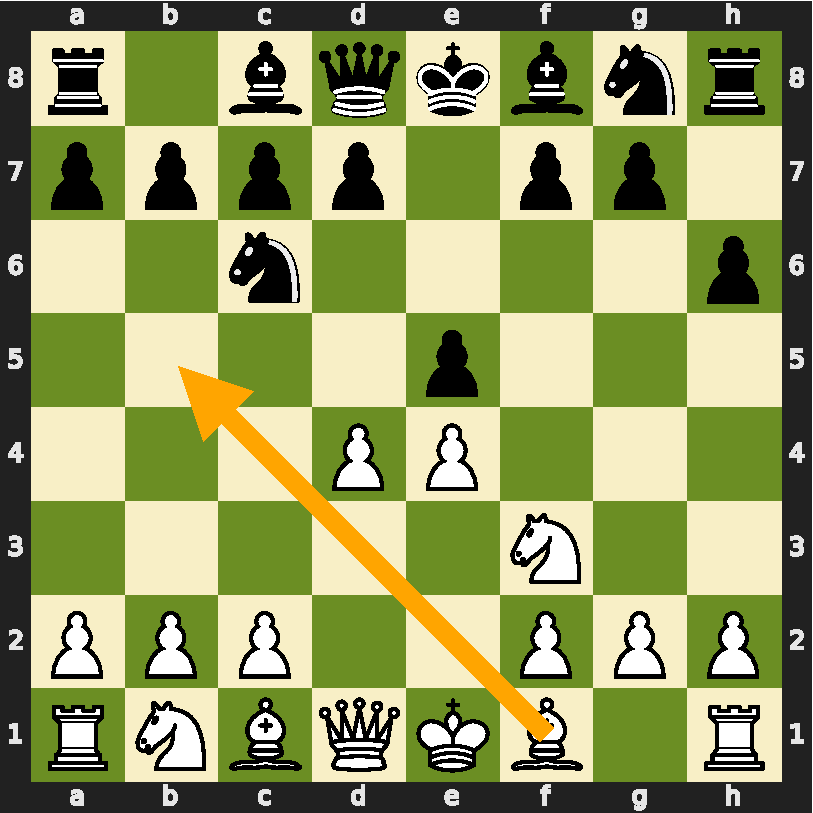
\includegraphics[width=\linewidth]{figures/board_prev.pdf}
\end{subfigure}
\hspace*{\fill}
\begin{subfigure}{0.43\textwidth}
   \vspace{.2in}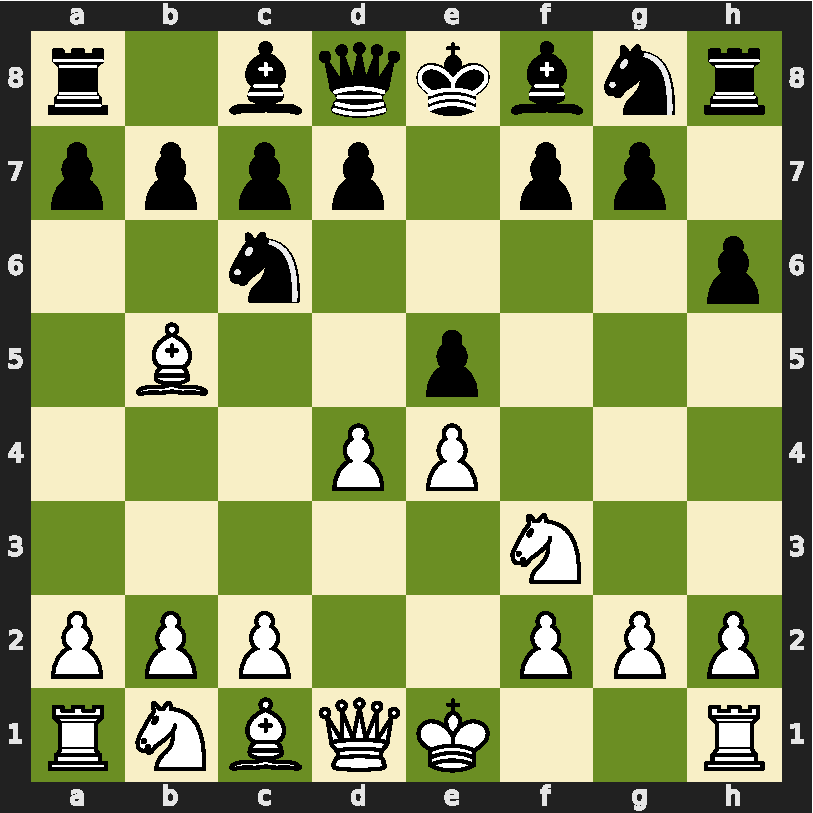
\includegraphics[width=\linewidth]{figures/board_next.pdf}
\end{subfigure}
\vspace{.1in}
\caption{Board state before (left) and after (right) the bishop at \pos{f1} is moved to \pos{b5}. UCI notation represents the move as \pos{f1b5}.}
\label{fig:move_notation}
\end{subfigure}
\vspace{-0.05in}
\caption{
Chess Notation %
}
\end{figure*}
